%%% Setup %%%
\documentclass{article}
\usepackage{fullpage}
\usepackage{graphicx}
\graphicspath{ {./} }
\title{Review of ``Computational Sprinting'' \cite{sprinting}}
\author{Riley Wood}
\begin{document}
\maketitle

%%% The Meat %%%

\section*{Key Ideas}
Because recently chip voltage has failed to scale down at the same rate as
transistor size, CPU power density has begun to increase. Without a means to
cool hotter and hotter chips, architects are forced to power down large areas of
the chip such that only small portions can be used at any a given time. This trend has been
coined "dark silicon" because it more and more transistors on chip must remain
unpowered or "dark" as they get smaller. This impacts mobile devices especially
which are more difficult to cool. The paper discusses one way of getting around
the utilization wall imposed by power limitations: exceed the thermal limits
only in short bursts to get more work done per unit time, when needed. They
mention interactive applications as their main target for improvement. These
applications generally spend a lot of time idle, waiting for user input,
punctuated by bursts of computation when input is received. They discuss
implications of computational sprinting for thermal, electrical, and software
design.

\section*{Review}
I looked at the paper they cite \cite{40} as evidence of the burstiness of most
mobile workloads. Figure 7 in that paper gives a breakdown of the power
consumption of a mobile phone.

\begin{figure}[h!]
    \centering
    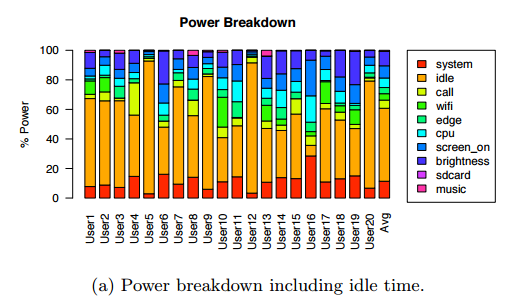
\includegraphics[width=7cm]{mobile_workload_breakdown}
\end{figure}

This is very convincing evidence, as one can see that idle times dominate power
consumption. A criticism I have is when they claim that delays longer than one
second "typically degrade the user experience" with no citation. Other papers
they cite, such as \cite{45}, aim to reduce computer response time below the
human-perceptual threshold of 50 to 100 milliseconds. It would be more
convincing if they provided a justification for why a delay of as much as one
second is reasonable. I also am weary of their suggestion of cooling the chip
with a material that melts at the chip's critical temperature, allowing it to
hold that temperature for an extended period of time (until the material has
fully melted). Their idea would be more convincing if they cited related work
(even tangentially related) as proof that the proposed solution involving a PCM
is feasible. I can imagine many things going wrong with this approach, such as
if the phase change material were to leak. As for the benchmarks used to test
the increase in responsiveness, it would be more convincing if they explained
how these benchmarks are analogous to typical interactive workloads users
perform on their phones, as these are the applications these researchers want to
make more responsive, at the end of the day. They mention that feature
extraction is similar to an image search one might do on their phone, but the
reader is left without an explanation as to why the others were chosen.

\section*{Conclusion}
I believe they make a good case for the potential benefit sprinting would offer,
given the bursty nature of mobile applications which they prove very well. It's
clear that they don't have a fleshed out solution for how to design chip
packages to allow sprinting. The PCM idea is interesting, but could use further
testing and validation. I would be interested to see future work that
investigates such a method of cooling a chip. I also believe they rely too
heavily on the idea that an acceptable response time is anything below one
second - a number that does not seem to be based on previous work. Still, I
suppose their work shows that through sprinting, a parallelizable workload can
be sped up by a factor of five. Wherever the line is drawn between unresponsive and responsive, it's possible
that sprinting might bring a workload below this threshold.

%%% References %%%
\bibliographystyle{unsrt}
\bibliography{sprinting}

%%% The End %%%
\end{document}
